Die wesentlichen Schritte im digitalen Signaturgsprozess sind signieren, verschlüsseln und prüfen mittels des asymmetrischen Schlüssel Konzepts. Das asymmetrische Schlüssel Konzept besteht aus der Generierung eines öffentlichen Schlüssels, dieser wird in einer Zertifizierungsstelle hinterlegt, und einem privaten Schlüssel, diesen besitzt der Signaturschlüssel-Inhaber, welcher auf einer Chipkarte vor Manipulationen geschützt ist und nicht verändert werden kann. \cite{techno1} 
\begin{figure}[!ht]
    \centering
    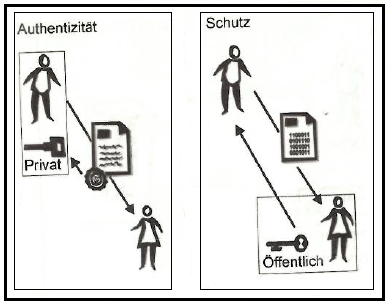
\includegraphics[height=260pt, width=350pt]{ablauf_async.PNG}
    \caption[Asymmetrisches Schlüssel Konzept]{\small{Asymmetrisches Schlüssel Konzept \cite{techno5}}}
\end{figure}